\documentclass{article}
\usepackage{amsmath}
\usepackage{tikz}
\usetikzlibrary{arrows.meta, decorations.pathreplacing}

\begin{document}

\begin{figure}[h]
    \centering
    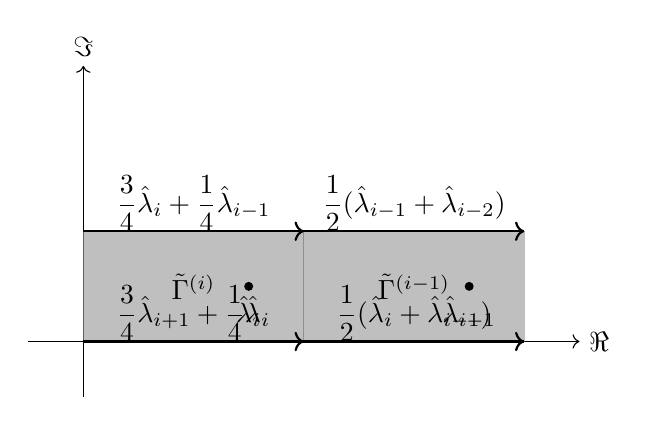
\begin{tikzpicture}[scale=0.7]
        % Axes
        \draw[->] (-1,0) -- (9,0) node[right] {$\Re$};
        \draw[->] (0,-1) -- (0,5) node[above] {$\Im$};
        
        % Curves
        \filldraw[gray, opacity=0.5] (0,0) rectangle (4,2);
        \filldraw[gray, opacity=0.5] (4,0) rectangle (8,2);
        
        % Labels for curves
        \node at (2,1) {\(\tilde\Gamma^{(i)}\)};
        \node at (6,1) {\(\tilde\Gamma^{(i-1)}\)};
        
        % Points within curves
        \filldraw (3,1) circle (2pt) node[below] {\(\hat{\lambda}_i\)};
        \filldraw (7,1) circle (2pt) node[below] {\(\hat{\lambda}_{i-1}\)};
        
        % Arrows
        \draw[->, thick] (0,0) -- (4,0);
        \draw[->, thick] (4,0) -- (8,0);
        \draw[->, thick] (0,2) -- (4,2);
        \draw[->, thick] (4,2) -- (8,2);
        
        % Long horizontal lines
        \draw[thick] (0,2) -- (8,2);
        \draw[thick] (0,0) -- (8,0);
        
        % Midpoints
        \node at (2,2.5) {\(\dfrac{3}{4}\hat{\lambda}_{i} + \dfrac{1}{4}\hat{\lambda}_{i-1}\)};
        \node at (6,2.5) {\(\dfrac{1}{2}(\hat{\lambda}_{i-1} + \hat{\lambda}_{i-2})\)};
        \node at (2,0.5) {\(\dfrac{3}{4}\hat{\lambda}_{i+1} + \dfrac{1}{4}\hat{\lambda}_{i}\)};
        \node at (6,0.5) {\(\dfrac{1}{2}(\hat{\lambda}_{i} + \hat{\lambda}_{i-1})\)};
    \end{tikzpicture}
    \caption{Choice of the curves \(\tilde\Gamma^{(i)}\) and \(\tilde\Gamma^{(i-1)}\) in the proof of Theorem \ref{Theorem2.3.1}.}
    \label{fig:CurvesChoice}
\end{figure}

\end{document}